\documentclass[border=2mm]{standalone}
\usepackage{tikz}
\usepackage{mathtools}
% \usepackage{tikz-3dplot}
\usetikzlibrary{calc}

\begin{document}
% \tdplotsetmaincoords{70}{120}

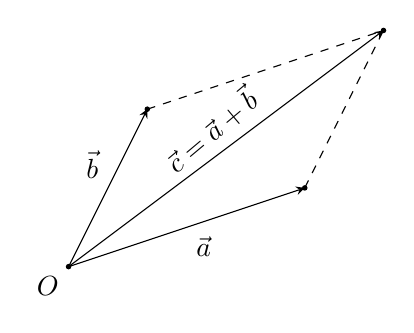
\begin{tikzpicture}[>=stealth]
  \coordinate (O) at (0,0);
  \coordinate (A) at (3,1);
  \coordinate (B) at (1,2);
  \coordinate (C) at ($(A)+(B)$);

  \draw[->] (O) -- (A) node[midway, below right] {$\vec{a}$};

  \draw[->] (O) -- (B) node[midway, above left] {$\vec{b}$};

  \draw[dashed] (A) -- (C);

  \draw[dashed] (B) -- (C);

  \draw[->] (O) -- (C) node[midway, above, rotate=40] {$\vec{c}=\vec{a} + \vec{b}$};

  \fill (O) circle (1pt) node[below left] {$O$};
  \fill (A) circle (1pt);
  \fill (B) circle (1pt);
  \fill (C) circle (1pt);
\end{tikzpicture}

\end{document}